%%%%%%%%%%%%%%%%%%%%%%%%%%%%%%%%%%%%%%%%%%%%%%%%%%%%%%%
% MatPlotLib and Random Cheat Sheet
%
% Edited by Michelle Cristina de Sousa Baltazar
%
% http://matplotlib.org/api/pyplot_summary.html
% http://matplotlib.org/users/pyplot_tutorial.html
%
%%%%%%%%%%%%%%%%%%%%%%%%%%%%%%%%%%%%%%%%%%%%%%%%%%%%%%%

\documentclass[a4paper]{article}
\usepackage[landscape]{geometry}
\usepackage{url}
\usepackage{multicol}
\usepackage{amsmath}
\usepackage{amsfonts}
\usepackage{tikz}
\usetikzlibrary{decorations.pathmorphing}
\usepackage{amsmath,amssymb}
\usepackage{hyperref}

\usepackage{colortbl}
\usepackage{xcolor}
\usepackage{mathtools}
\usepackage{amsmath,amssymb}
\usepackage{enumitem}

% Mihnea
\usepackage{textcomp} % \textquotesingle: Racket: '(1 2 3)
\usepackage{couriers}
\usepackage{listings}
\lstset{
    numbers         = left,
    numberstyle     = \tiny,
    numbersep       = 5pt,
    captionpos      = b,
    breaklines      = true,
    basicstyle      = \ttfamily\footnotesize, 
    tabsize         = 4,
    escapeinside    = {~}{~},
}
\lstdefinelanguage{Racket}{
  morekeywords=[1]{define, define-syntax, define-macro, lambda, define-stream, stream-lambda},
  morekeywords=[2]{begin, call-with-current-continuation, call/cc,
    call-with-input-file, call-with-output-file, case, cond,
    do, else, for-each, if,
    let*, let, let-syntax, letrec, letrec-syntax,
    let-values, let*-values,
    and, or, not, delay, force,
    quasiquote, quote, unquote, unquote-splicing,
    map, fold, syntax, syntax-rules, eval, environment },
  morekeywords=[3]{import, export},
  alsodigit=!\$\%&*+-./:<=>?@^_~,
  sensitive=true,
  morecomment=[l]{;},
  morecomment=[s]{\#|}{|\#},
  morestring=[b]",
  basicstyle=\footnotesize\ttfamily,
  keywordstyle=\color[rgb]{0,.3,.7},
  commentstyle=\color[rgb]{0.133,0.545,0.133},
  stringstyle={\color[rgb]{0.75,0.49,0.07}},
  upquote=true,
  breaklines=true,
  breakatwhitespace=true,
  literate=*{`}{{`}}{1}
}

\title{Racket-2}
\usepackage[romanian]{babel}
\usepackage[utf8]{inputenc}

\advance\topmargin-1.0in
\advance\textheight3in
\advance\textwidth3in
\advance\oddsidemargin-1.5in
\advance\evensidemargin-1.5in
\parindent0pt
\parskip1pt
\newcommand{\hr}{\centerline{\rule{3.5in}{1pt}}}
%\colorbox[HTML]{e4e4e4}{\makebox[\textwidth-2\fboxsep][l]{texto}
\begin{document}

\begin{center}{\huge{\textbf{Racket CheatSheet}}}\\
{\large Laborator 3}
\end{center}
\begin{multicols*}{3}

\tikzstyle{mybox} = [draw=black, fill=white, very thick,
    rectangle, rounded corners, inner sep=10pt, inner ysep=9pt]
\tikzstyle{fancytitle} =[fill=black, text=white, font=\bfseries]

% Mihnea
\tikzstyle{mybox_code} = [mybox, draw = orange, fill=sandybrown]
\tikzstyle{fancytitle_code} = [fancytitle, fill = orange]

\definecolor{almond}{rgb}{0.94, 0.87, 0.8}
\definecolor{apricot}{rgb}{0.98, 0.81, 0.69}
\definecolor{atomictangerine}{rgb}{1.0, 0.6, 0.4}
\definecolor{sandybrown}{rgb}{0.96, 0.64, 0.38}
\definecolor{buff}{rgb}{0.94, 0.86, 0.51}

\definecolor{persianred}{rgb}{0.8, 0.2, 0.2}
\definecolor{papayawhip}{rgb}{1.0, 0.94, 0.84}
\tikzstyle{mybox_persianred} = [mybox, draw = persianred, fill=papayawhip]
\tikzstyle{fancytitle_persianred} = [fancytitle, fill = persianred]

\definecolor{whitesmoke}{rgb}{0.96, 0.96, 0.96}
\definecolor{wenge}{rgb}{0.39, 0.33, 0.32}
\tikzstyle{mybox_blue} = [mybox, draw = wenge, fill=whitesmoke]
\tikzstyle{fancytitle_blue} = [fancytitle, fill = wenge]

\definecolor{cerise}{rgb}{0.87, 0.19, 0.39}
\definecolor{mistyrose}{rgb}{1.0, 0.89, 0.88}
\tikzstyle{mybox_cerise} = [mybox, draw = cerise, fill=mistyrose]
\tikzstyle{fancytitle_cerise} = [fancytitle, fill = cerise]

\definecolor{pinegreen}{rgb}{0.0, 0.47, 0.44}
\definecolor{bubbles}{rgb}{0.91, 1.0, 1.0}
\tikzstyle{mybox_pinegreen} = [mybox, draw = pinegreen, fill=bubbles]
\tikzstyle{fancytitle_pinegreen} = [fancytitle, fill = pinegreen]

\definecolor{cream}{rgb}{1.0, 0.99, 0.82}
\definecolor{mikadoyellow}{rgb}{1.0, 0.77, 0.05}
\tikzstyle{mybox_mikadoyellow} = [mybox, draw = mikadoyellow, fill=cream]
\tikzstyle{fancytitle_mikadoyellow} = [fancytitle, fill = mikadoyellow]

\definecolor{cornsilk}{rgb}{1.0, 0.97, 0.86}
\tikzstyle{mybox_orange} = [mybox, draw = orange, fill=cornsilk]
\tikzstyle{fancytitle_orange} = [fancytitle, fill = orange]

\definecolor{aliceblue}{rgb}{0.94, 0.97, 1.0}
\definecolor{seagreen}{rgb}{0.18, 0.55, 0.34}
\tikzstyle{mybox_seagreen} = [mybox, draw = seagreen, fill=aliceblue]
\tikzstyle{fancytitle_seagreen} = [fancytitle, fill = seagreen]

\definecolor{jazzberryjam}{rgb}{0.65, 0.04, 0.37}
\definecolor{almond}{rgb}{0.94, 0.87, 0.8}
\tikzstyle{mybox_jazzberryjam} = [mybox, draw = jazzberryjam, fill=almond]
\tikzstyle{fancytitle_jazzberryjam} = [fancytitle, fill = jazzberryjam]

\definecolor{amaranth}{rgb}{0.9, 0.17, 0.31}
\definecolor{bisque}{rgb}{1.0, 0.89, 0.77}
\tikzstyle{mybox_amaranth} = [mybox, draw = amaranth, fill=bisque]
\tikzstyle{fancytitle_amaranth} = [fancytitle, fill = amaranth]

\definecolor{carminered}{rgb}{1.0, 0.0, 0.22}
\definecolor{blanchedalmond}{rgb}{1.0, 0.92, 0.8}
\tikzstyle{mybox_carminered} = [mybox, draw = amaranth, fill=blanchedalmond]
\tikzstyle{fancytitle_carminered} = [fancytitle, fill = carminered]

\definecolor{midnightgreen}{rgb}{0.0, 0.29, 0.33}
\definecolor{lavendermist}{rgb}{0.9, 0.9, 0.98}
\tikzstyle{mybox_midnightgreen} = [mybox, draw = midnightgreen, fill=lavendermist]
\tikzstyle{fancytitle_midnightgreen} = [fancytitle, fill = midnightgreen]

\definecolor{indigo}{rgb}{0.29, 0.0, 0.51}
\definecolor{isabelline}{rgb}{0.96, 0.94, 0.93}
\tikzstyle{mybox_indigo} = [mybox, draw = indigo, fill=isabelline]
\tikzstyle{fancytitle_indigo} = [fancytitle, fill = indigo]

\definecolor{russet}{rgb}{0.5, 0.27, 0.11}
\definecolor{ivory}{rgb}{1.0, 1.0, 0.94}
\tikzstyle{mybox_russet} = [mybox, draw = russet, fill=ivory]
\tikzstyle{fancytitle_russet} = [fancytitle, fill = russet]

\definecolor{neongreen}{rgb}{0.22, 0.88, 0.08}
\definecolor{splashedwhite}{rgb}{1.0, 0.99, 1.0}
\tikzstyle{mybox_neongreen} = [mybox, draw = neongreen, fill=splashedwhite]
\tikzstyle{fancytitle_neongreen} = [fancytitle, fill = neongreen]

\tikzstyle{mybox_skyblue} = [mybox, draw = blue!60, fill=splashedwhite]
\tikzstyle{fancytitle_skyblue} = [fancytitle, fill = blue!60]



%-----------------------------------------------------------------------------
\begin{tikzpicture}
\node [mybox_midnightgreen] (box){%
    \begin{minipage}{0.3\textwidth}
    {\centering\bf\color{midnightgreen}    (lambda (arg1 arg2 ...) rezultat) \\ (define nume val) \\ }
% \[ CTRL\hspace{3pt}\backslash \hspace{10pt} \lambda \] \\

        \begin{lstlisting}[language=Racket]          
(lambda (x) x)                 functia identitate
((lambda (x) x) 2)          2  aplicare functie
(define idt (lambda (x) x))    legare la un nume
(define (idt x) x)             sintaxa alternativa
(idt 3)                     3

((if true + -) (+ 1 2) 3)   6  ~if-ul se evaluează~
                               ~la o funcție~
                               
(define (comp f g)             ~funcția de~
  (lambda (x)                  ~compunere ($\circ$)~
    (f (g x))))                ~a altor 2 funcții~
    
((comp car cdr) '(1 2 3))   2  ~car $\circ$ cdr~

((comp (lambda (x) (+ x 1)) 11 ~inc $\circ$ dublare~
       (lambda (x) (* x 2)))
 5)
        \end{lstlisting}\vspace*{-2ex}
    \end{minipage}
};

\node[fancytitle_midnightgreen, right=10pt] at (box.north west) {Funcții anonime (lambda) și funcții cu nume};
\end{tikzpicture}

\begin{tikzpicture}
\node [mybox_seagreen] (box){%
    \begin{minipage}{0.3\textwidth}     
        \begin{lstlisting}[language=Racket]
(define add-uncurried          ~parametri luați~
  (lambda (x y)                ~simultan~
    (+ x y)))
    
(add-uncurried 1 2)         3

(define add-curried            ~parametri luați~
  (lambda (x)                  ~succesiv~
    (lambda (y)
      (+ x y))))
      
((add-curried 1) 2)         3

(define inc (add-curried 1))   ~aplicație parțială~
        \end{lstlisting}
        
        Perspective asupra funcțiilor binare \emph{curried}:
        \begin{itemize}\itemsep0ex
            \item Iau parametrii „pe rând”, fiind aplicabile parțial.
            
            \item Iau un parametru și întorc o altă funcție de un parametru.
        \end{itemize}
    \end{minipage}
};

\node[fancytitle_seagreen, right=10pt] at (box.north west) {Funcții \emph{curried}/ \emph{uncurried}};
\end{tikzpicture}

\begin{tikzpicture}
\node [mybox_orange] (box){%
    \begin{minipage}{0.3\textwidth}
        {\centering\bf\color{orange} (filter funcție listă) \\}
        \vskip5pt
        Păstrează dintr-o listă elementele pentru care funcția NU întoarce \texttt{false}.
        $\tt (filter~f~(list~e_1~\ldots~e_n)) \to (list~e_{i_1}~\ldots~e_{i_m})$,
        cu $\tt (f~e_{i_k}) \not \to false$.
        \begin{lstlisting}[language=Racket]
(filter even? '(1 2 3))                 '(2)
        \end{lstlisting}\vspace*{-1ex}
    \end{minipage}
};

\node[fancytitle_orange, right=10pt] at (box.north west) {Funcționala \texttt{filter}};
\end{tikzpicture}

\begin{tikzpicture}
\node [mybox_indigo] (box){%
    \begin{minipage}{0.3\textwidth}
        {\centering\bf\color{indigo} (fold* funcție acumulator listă) \\
         funcție $\to$ (lambda (element acumulator') acumulator'') \\}
         \vskip5pt
        Îmbină toate elementele unei liste pentru a construi o valoare finală, pornind
        de la un acumulator inițial. Într-un pas, funcția dată ca parametru combină 
        elementul curent din listă cu acumulatorul, întorcând un nou acumulator. 
        Acumulatorul final este întors ca rezultat al funcționalelor \texttt{fold*}.
        Acesta poate fi chiar o listă.
        \begin{itemize}
            \item \texttt{foldr} (\emph{right}) poate fi înțeleasă cel mai ușor prin faptul 
                că funcția dată ca parametru se substituie lui \texttt{cons}, iar 
                acumulatorul inițial, listei vide de la finalul listei. Prin urmare, 
                elementele listei sunt prelucrate de la dreapta la stânga:
                $\tt (foldr~f~acc~(list~e_1~\ldots~e_n)) \to (f~e_1~(f~\ldots~(f~e_n~acc)\ldots))$
                
            \item \texttt{foldl} (\emph{left}) prelucrează elementele de la stânga la dreapta:
            $\tt (foldl~f~acc~(list~e_1~\ldots~e_n)) \to (f~e_n~(f~\ldots~(f~e_1~acc)\ldots))$
        \end{itemize}
        Se pot furniza mai multe liste, caz în care comportamentul este similar cu cel al lui \texttt{map}
        pe mai multe liste.
        \begin{lstlisting}[language=Racket]
(foldr + 0 '(1 2 3))  6 ~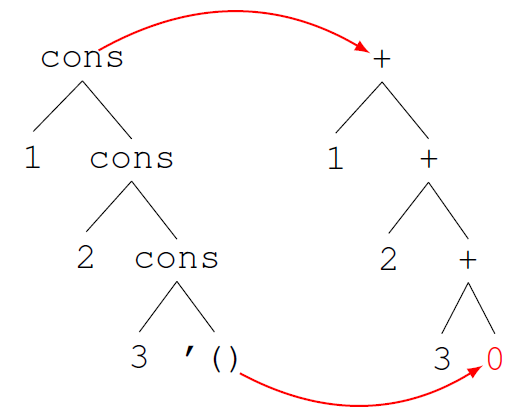
\includegraphics[scale=0.3]{imgs/foldr}~
(foldl + 0 '(1 2 3))  6 ~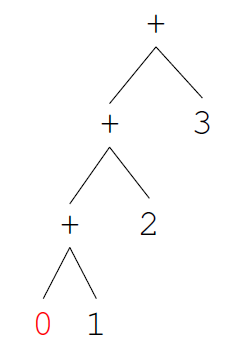
\includegraphics[scale=0.32]{imgs/foldl}~
(foldr cons '() '(1 2 3))   '(1 2 3)   ~identitate!~
(foldl cons '() '(1 2 3))   '(3 2 1)   ~inversare~
(foldl (lambda (x y acc)          21   ~2 liste~
         (+ x y acc))
       0 '(1 2 3) '(4 5 6))       
        \end{lstlisting}
    \end{minipage}
};

\node[fancytitle_indigo, right=10pt] at (box.north west) {Funcționalele \texttt{foldl} și \texttt{foldr}};
\end{tikzpicture}


\begin{tikzpicture}
\node [mybox_persianred] (box){%
    \begin{minipage}{0.3\textwidth}
        {\centering\bf\color{persianred} (map funcție listă) \\ (map funcție lista1 lista2 ...) \\}
        \vskip5pt
        Transformă independent elementele de pe poziții diferite ale uneia sau mai multor liste.
        Întoarce o listă cu același număr de elemente ca lista/ listele date ca parametru.
        \begin{itemize}
            \item Pentru o singură listă, aplică funcția, pe rând  asupra fiecărui element:
                $\tt (map~f~(list~e_1~\ldots~e_n)) \to (list~(f~e_1)~\ldots~(f~e_n))$
            
            \item Pentru mai multe liste de aceeași lungime, funcția este aplicată la un moment dat asupra tuturor  
                elementelor de pe aceeași poziție:
                $\tt (map~f~(list~e_{11}~\ldots~e_{1n})~\ldots~(list~e_{m1}~\ldots~e_{mn}))
                \to (list~(f~e_{11}~\ldots~e_{m1})~\ldots~(f~e_{1n}~\ldots~e_{mn}))$
        \end{itemize}
        Există și funcționalele \texttt{andmap} și \texttt{ormap}. Prima se asigură că, în urma aplicării lui 
        \texttt{map}, toate rezultatele sunt diferite de \texttt{false}, iar a doua, că cel puțin un rezultat
        este diferit de \texttt{false}.
        \begin{lstlisting}[language=Racket]
(map (lambda (x) (* x 10)) '(1 2 3))   '(10 20 30)
(map * '(1 2 3) '(10 20 30))           '(10 40 90)
(map list '(1 2 3))                 '((1) (2) (3))
(map list '(1 2) '(3 4))            '((1 3) (2 4))

(define (mult-by q)                      ; Curried
  (lambda (x)
    (* x q)))
(map (mult-by 5) '(1 2 3))              '(5 10 15)
        \end{lstlisting}
    \end{minipage}
};

\node[fancytitle_persianred, right=10pt] at (box.north west) {Funcționala \texttt{map}};
\end{tikzpicture}

%\vskip50ex % pentru a trece la următoarea coloană

%-----------------------------------------------------------------------------
%\vskip50ex % pentru a trece la următoarea coloan

%-----------------------------------------------------------------------------
\begin{tikzpicture}
\node [mybox_russet] (box){%
    \begin{minipage}{0.3\textwidth}
        {\centering\bf\color{russet} (apply funcție listă\_arg) \\ (apply funcție arg\_1 ... arg\_n listă\_arg) \\}
        \vskip5pt
        Aplică o funcție asupra parametrilor dați de elementele unei liste. Opțional, primii parametri ai funcției 
        îi pot fi furnizați individual lui \texttt{apply}, înaintea listei cu restul parametrilor.
        $\tt (apply~f~x_1~\ldots~x_m~(list~e_1~\ldots~e_n)) \to (f~x_1~\ldots~x_m~e_1~\ldots~e_n)$
        \begin{lstlisting}[language=Racket]
(apply + '(1 2 3))              6         ~suma~
(apply + 1 '(2 3))              6         ~la fel~
(apply list '(1 2 3))           '(1 2 3)
(apply list '(1 2 3) '(5 6 7))  '((1 2 3) 5 6 7)
        \end{lstlisting}
    \end{minipage}
};

\node[fancytitle_russet, right=10pt] at (box.north west) {Funcționala \texttt{apply}};
\end{tikzpicture}

%-----------------------------------------------------------------------------


\end{multicols*}
\end{document}
Contact GitHub API Training Shop Blog About
© 2016 GitHub, Inc. Terms Privacy Security Status Help